\subsubsection*{Cost Category 22.01.03: Coils}

This cost category includes the costing for the plasma confinement coils, including  material, structural and manufacturing cost. As a primary cost driver for this device, careful consideration of a number of parameters is taken, including the number of coils, the B$\cdot$R value ( in the case of the solenoid coils here), the conductor material, winding type, and quench mitigation in the case of superconducting cables.\\

Consists of:

\begin{itemize}
    \item 22.1.3.1 Solenoid coils
    \item 22.1.3.2 Mirror coils
    \item 22.1.3.3
    \item 22.1.3.4 Shim coils
    \item 22.1.3.5 Structural support
    \item 22.1.3.6 Cryogenic system
\end{itemize}
   

The approach taken was to compare various geometries of HTS, LTS and copper coil sets using COMSOL, with the same central field and minimum inner radius requirements. These were down-selected to an HTS geometry with noCoil1Coils solenoid coils, and noCoil2Coils inner mirror coils and noCoil3Coils outer mirror coils.\\

To determine the cost, the coil parameters were determined using a combination of COMSOL, calibration points from the literature including Menard 2016 \cite{Menard2016} for HTS, and EU DEMO for LTS, and analytical electromagnetic modeling. The material cost then then be determined through the mass/length (in the case of REBCO tape) of each material used. 

To cost the magnet system, two steps are required. The first is to have the specifications of the magnets required, and the second is to calculate the resulting material requirements and costs, with a manufacturing factor applied to this total. In the costing code provided, four basic magnet types are available: HTS (CICC), HTS (pancake), LTS (CICC) and copper. In the standard code, as arguably the new industry standard, only HTS (CICC) includes both both steps of design and costing. For all others, the user will need to provide the following basic specifications to input into the code for a cost to be returned:

\begin{itemize}
    \item Magnet coil counts: this input specifies the number of identical coils of each type.
    \item Magnet type: specifies the magnet type of the four described above.
    \item \textit{r} centre: the average radius of the coil.
    \item \textit{z} centre: the displacement of the centre of the coil in the \textit{z} (vertical) axis.
    \item \textit{dr}: the radial thickness of each coil.
    \item \textit{dz}: the thickness of each coil in the \textit{z} axis.
    \item Insulating material fraction: in the case of the pancake winding geometry, a "partial insulation" is used. Currently, the 'partial insulation' technology being developed by, for example, Tokamak Energy is proprietary and details are not publicly available. As such, for costing purposes, a fraction of fracIns of the total cross-sectional area is assumed to be insulating material, with a density similar to paraffin or epoxy, and a material cost of mcostI \$/kg. These values are purely indicative of an order-of-magnitude costing reference, and can be updated with more information as costing code inputs.
    \item Manufacturing factor: a scalar multiplying factor which is applied to the total material cost of each coil, based upon the complexity and cost of winding and installing the coil. Default values are provided for each coil type. For HTS, for example, there has yet to be a commercially implemented CICC, so it is assumed that the cost of winding is comparable with that of LTS, which is widely available. 
    \item Structural factor: another scalar multiplying factor applied to the total cost of the magnet (including manufacturing factor). This accounts for the direct structure required to support each magnet. Default values are provided here too, varying approximatley from 25-100\% of the base cost of the magnet.
\end{itemize}

For the purposes of clarity, and as a methodology guide for other coil types, the design approach for step 1 of the HTS (CICC) coils is as follows. The coil geometries and specifications as described in Menard 2016 \cite{Menard2016} as used as a calibration point. These specifications are then input into a Biot-Savart code that calculates the field at given coordinates. The coil is considered to comprise of N turns of current-carrying circular loops, with varying radii and \textit{r} and \textit{z} displacements. The total contributions of each concentric turn are then summed to determine the central field at \textit{r = 0}.

Using these data, a SciPy interpolation function is used to determine the coil specifications required to achieve a given central field, constrained by the required average radius.

It should be noted that the default cable geometry as seen in \href{fig:yuhu_cs} is by no means optimised, and it is recommended that for minimal capital costs, a minimal length of REBCO and a maximum available current is used.


\begin{figure}[h]
    \centering
    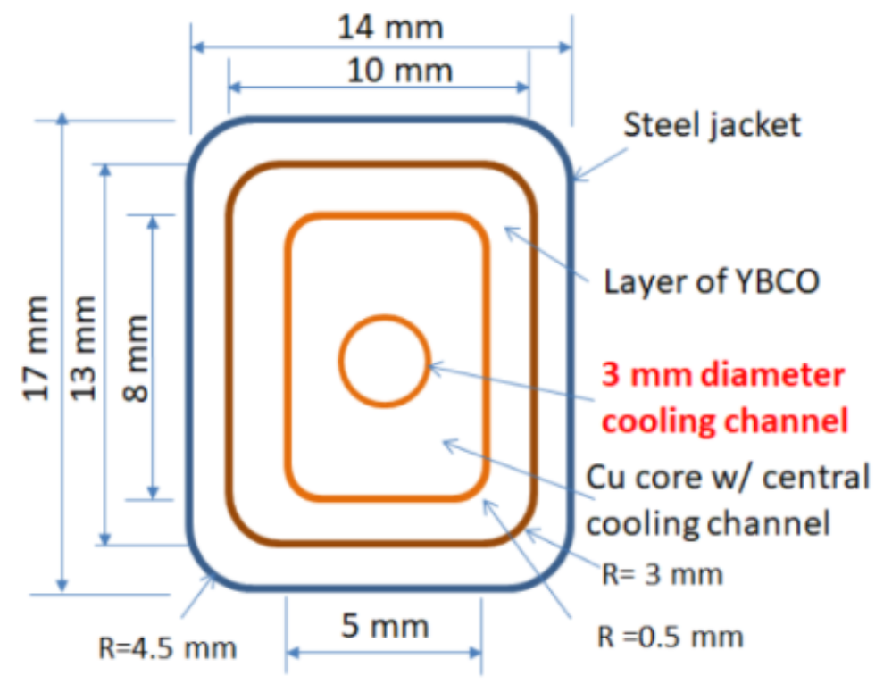
\includegraphics[width =0.5\linewidth]{StandardFigures/yuhu_cs.pdf}
    \caption{HTS cable geometry.}
    \label{fig:yuhu_cs}
\end{figure}

Another recommended approach is to employ a multi-physics FEM tool such as COMSOL to design the magnet with the required properties to obtain the inputs required for the costing code.

It should be noted that a series of optimizations can be made to the design to reduce cost. The first of these is conductor grading. By reducing the number of strands of superconductor where the fields lower, up to 50\% of the superconducting material can be saved \cite{uglietti2018progressing}.\\

The total cost of the coils is C220103 M USD.


\subsubsection*{22.1.3.1 Solenoid coils}

This design consists of notfcoils solenoid coils, which can be individually removed for maintenance. The total cost is C22010302 M USD.\\

Both LTS and HTS cables can be considered here. For each, a wide variety of designs are available, including no-insulation, partial insulation, and an array of CICC geometries. For this concept, a simple CICC geometry is considered \cite{Menard2016}, comprising a layer of superconducting REBCO conductor, copper for quench mitigation and cooling, a central coolant channel, and a steel jacket to help resist the considerable forces experienced during operation. See \ref{fig:yuhu_cs} for the specific geometry.\\

To cost the system, the magnet specifications are calibrated against \cite{Menard2016}, and extrapolated to the requirements of this concept. The total length of the conductor is then calculated and, assuming a cost of 12 \$/kAm, the total cost can be found. For the steel and copper, the volume is also found and multiplied by the cost per kilogram. This gives a total material cost for the coil, which is then multiplied by a manufacturing factor. The manufacturing factor comprises the cost of manufacturing the cables, then winding and installing the coils. \\

The total cost of the solenoid coils is C22010301 M USD.


\subsubsection*{22.1.3.2 Mirror Coils}

This subsystem includes a large set of 20T HTS mirror coils at each end of the system. This central field strength is not achievable with copper magnets, meaning that HTS and LTS coils must be considered here. In this case, HTS coils are used, owing to their significantly increased current density, reducing the required number of turns and length of superconductor. This allows for a reduced form factor for the entire system, resulting in a multiplicative cost saving. In the case of the HTS magnets used in this system, a simple 'pancake' geometry is used, omitting the external conduit used in CICC geometries such as the VIPER or CORC cables. Instead, a "partial insulation" is used. Currently, the 'partial insulation' technology being developed by, for example, Tokamak Energy is proprietary and details are not publicly available. As such, for costing purposes, a fraction of fracIns of the total cross-sectional area is assumed to be insulating material, with a density similar to paraffin or epoxy, and a material cost of mcostI \$/kg. These values are purely indicative of an order-of-magnitude costing reference, and can be updated with more information as costing code inputs.

The total cost of the mirror coils is C22010302 M USD. \\


\subsubsection*{22.1.3.3}

There are only two main coil types in this magnetic mirror concept, so this cost category is obsolete in this case.


\subsubsection*{22.1.3.4 Shim Coils}

These coils serve to apply fine adjustments to the field profile to maintain field uniformity, and control any plasma disturbances. The placement, size, and magnitude of these coils is dependent upon the uniformity requirements of the plasma, and requires sophisticated FEM analysis to accurately quantify. As such, for the scope of this costing report, a simple factor of 5\% of the total primary magnet costs is taken. The resulting cost is C22010304 M USD.\\

\begin{table}[h]
\centering
\resizebox{\linewidth}{!}{%
\begin{tabular}{lcccc}
\hline
\textbf{Parameter} & \textbf{Solenoid} & \textbf{M1} & \textbf{M2} \\
\hline
Magnet Type & magnetType1 & magnetType2 & magnetType3 \\
Radius (m) & rCentre1 & rCentre2 & rCentre3 \\
dr (m) & dr1 & dr2 & dr3 \\
dz (m) & dz1 & dz2 & dz3 \\
Current supply (MA) & currentSupply1 & currentSupply2 & currentSupply3 \\
Conductor current density (A/mm$^2$) & jTape1 & jTape2 & jTape3 \\
Cable width (m) & cableW1 & cableW2 & cableW3 \\
Cable height (m) & cableH1 & cableH2 & cableH3 \\
Total volume (m$^3$) & volCoil1 & volCoil2 & volCoil3 \\
Cross-sectional area (m$^2$) & csArea1 & csArea2 & csArea3 \\
Turn-turn Insulation Fraction & fracIns1 & fracIns2 & fracIns3 \\
\hline
Cable turns & turnsC1 & turnsC2 & turnsC3 \\
Total turns of conductor & turnsScTot1 & turnsScTot2 & turnsScTot3 \\
Length of conductor (km) & tapeLength1 & tapeLength2 & tapeLength3 \\
Current per conductor (A) & tapeCurrent1 & tapeCurrent2 & tapeCurrent3 \\
\hline
Cost of REBCO tape(\$/kAm) & mCostYBCO & mCostYBCO & mCostYBCO \\
Cost of SC (M USD) & costSC1 & costSC2 & costSC3 \\
Cost of copper (M USD) & costCu1 & costCu2 & costCu3 \\
Cost of SS (M USD) & costSS1 & costSS2 & costSS3 \\
Cost of other turn-turn insulation (M USD) & costI1 & costI2 & costI3 \\
Total material cost (M USD) & totMatCost1 & totMatCost2 & totMatCost3 \\
Manufacturing factor & mfrFactor1 & mfrFactor2 & mfrFactor3 \\
Structural cost (M USD) & SolenoidStructCost & M1StructCost & M2StructCost \\
Cooling power (MW) & Qin1 & Qin2 & Qin3 \\
Cooling cost (M USD) & coolingCost1 & coolingCost2 & coolingCost3 \\
Quantity & noSolenoidCoils & noM1Coils & noM2Coils3 \\
Magnet cost (single)(M USD) & SolenoidMagCost & M1MagCost & M2MagCost \\
Magnet + structure cost (single) (M USD) & totalSolenoidCostI & totalM1CostI & totalM2CostI \\
\hline
Total cost (M USD) & totalSolenoidCost & totalM1Cost & totalM2Cost \\
\hline
\end{tabular}}
\caption{Design parameters for an individual coil of each of the main coils in this concept.}
\label{your-table-label}
\end{table}



\subsubsection*{22.1.3.5 Structural cost for coils}

The structural cost for the coils is difficult to cost from first principles without detailed structural analysis with FEM. Here, the approach is a series of analytical estimations of the dominant stresses. These include:

\begin{itemize}
    \item Hoop stress within the coil generated by the cumulative effect of the induced force between concentric radial turns.
    \item Axial force generated between cable turns within the coils. 
    \item Axial force between adjacent coils.
\end{itemize}


By considering these primary contributions, an estimate of the structural material required (such as the hoop restraint requirements) can be calculated. From this preliminary estimate, a structural cost of 25\% of the coil cost is used as a conservative factor. This is in comparison to 50-100\% as the standard for Tokamaks. The structural cost is thus C22010305 M USD.


\subsubsection*{22.1.3.6 Helium Liquefier-Refrigerators }This subsystem is the helium refrigeration and liquefaction process equipment. It is responsible for supplying the cooling necessary to maintain an operation temperature of 20 K in the chamber. \\

To determine the cooling power necessary to maintain 20 K in the coils, an analytical approach is taken, considering the primary heating components at the HTS coils. These are assumed to be the heat conducted through the support structure, and the neutron flux through the blanket (assuming 99\% of the neutron power is captured in the blanket). At 20 K, for one coil, these are estimated to contribute 11.2 and 1.8 kW, respectively. Scaling for a refrigeration efficiency of 15\% of the Carnot efficiency between 300 and 20 K, this results in a room temperature cooling power requirement of Qin MW. The operation temperature is selected based on a trade-off of the cooling efficiency (see fig \ref{fig:cool_eff}), and the superconducting properties of the HTS coils.\\

Using ITER as a reference, with learning curve credit applied, the cost for 47 kW of cooling at 4.2 K is 236 M USD. Scaling this to the cooling requirements of the system presented here results in a cost of C22010306 M USD. \\

\begin{figure}[h]
    \centering
    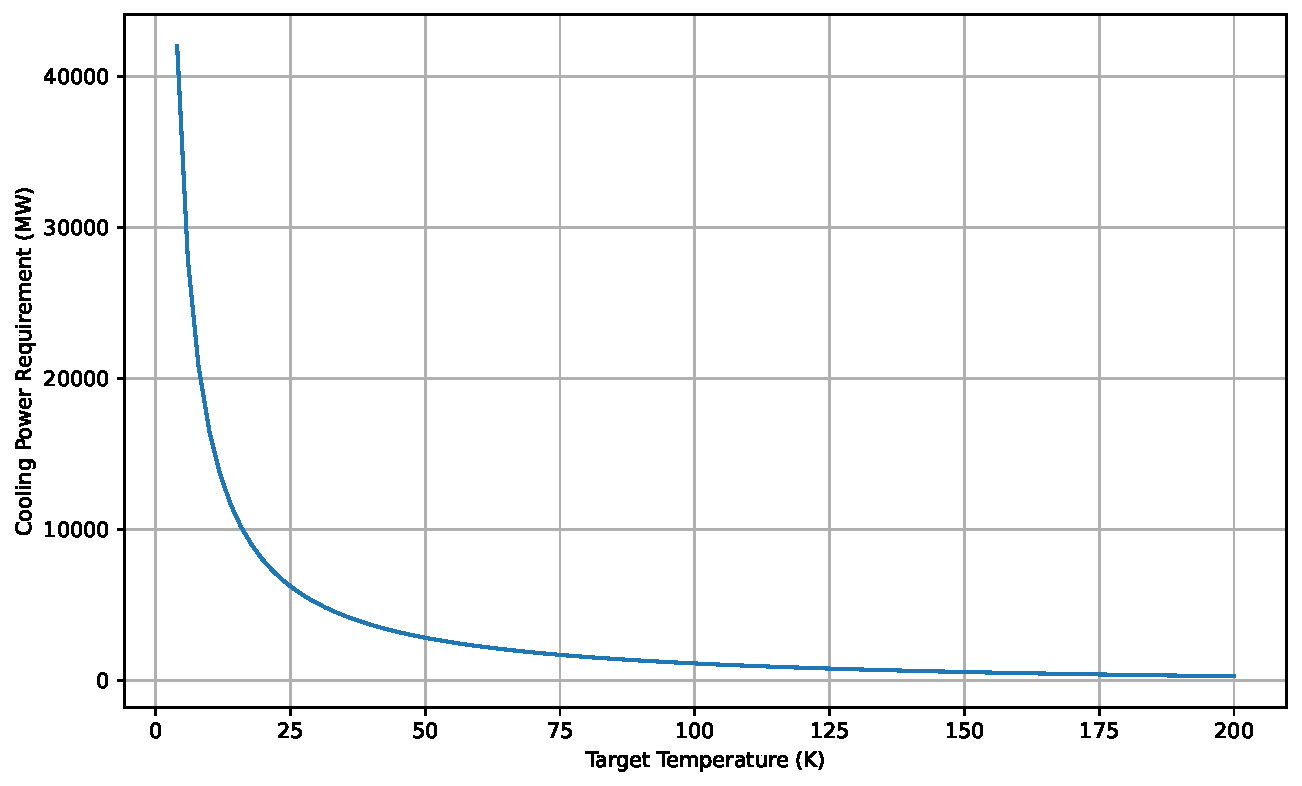
\includegraphics[width=0.75\linewidth]{Figures/cooling_efficiency.pdf}
    \caption{The cooling power requirement for various magnet operating temperatures.}
    \label{fig:cool_eff}
\end{figure}


